\documentclass{scrreprt}
\usepackage{hyperref}
\usepackage[dutch]{babel}
\usepackage[demo]{graphicx}
\usepackage{etoolbox}
\usepackage{float}
\usepackage[tocentry, tablegrid]{vhistory} 

%Remove newpage from chapter
\makeatletter
\patchcmd{\scr@startchapter}{\if@openright\cleardoublepage\else\clearpage\fi}{}{}{}
\makeatother
\DeclareGraphicsExtensions{.pdf,.png,.jpg}

\begin{document}
	\begin{titlepage}
		\centering
		{\scshape\LARGE Architectuur Document \par}
		\vspace{1cm}
		{\scshape\Large Team Gamma (C)\par}
		\vspace{1.5cm}
		{\huge\bfseries Rekeningrijden\par}
		\vspace{2cm}
		{\large\itshape Guus Hamm, Mathijn van Buul, Frank Hartman, Rick Rongen\par}
		\vfill
		% Bottom of the page
		{\large v\vhCurrentVersion\par}
		{\large \vhCurrentDate\par}
	\end{titlepage}
	\tableofcontents
	\newpage
	\begin{versionhistory}
		\vhEntry{0.1}{11-04-2017}{RR}{Initieel document}
	\end{versionhistory}

	\newpage
	\chapter{Inleiding}
	\section{Context}
		De overheid van Groot-Brittannië wil een nieuw stelsel invoeren waar de automobilisten betalen voor de hoeveelheid die zie rijden in plaats van het bezitten van een auto.\par
		Om dit te verwezenlijken is het team 'Team Gamma' ingeschakeld om dit te realiseren. 
	\section{Applicatie}
		De applicatie bestaat uit meerdere componenten die onderling communiceren. Deze zijn verantwoordelijk voor het rapporteren van de gereden kilometers, het verwerken hiervan en maandelijks een factuur sturen naar de gebruiker.
	\section{Niet-functionele eisen}
		Het is belangrijk dat minimaal het registratie gedeelte van de applicatie ten alle tijden beschikbaar is. Als dit niet werkt dan kunnen mensen 'gratis' rijden.\par
		Verder is het belangrijk dat de applicatie accuraat is, 
	\section{Doel van dit document}
		Het doel van dit document is om duidelijk het project weer te geven en alle onderdelen uit te leggen. Dit zodat na het doornemen van dit document het duidelijk is hoe het project in elkaar zit en hoe er aan gewerkt kan worden.
	
	\newpage
	\chapter{Domein Model}
	\section{Klassendiagram}
	\begin{figure}[ht]
		\centering
		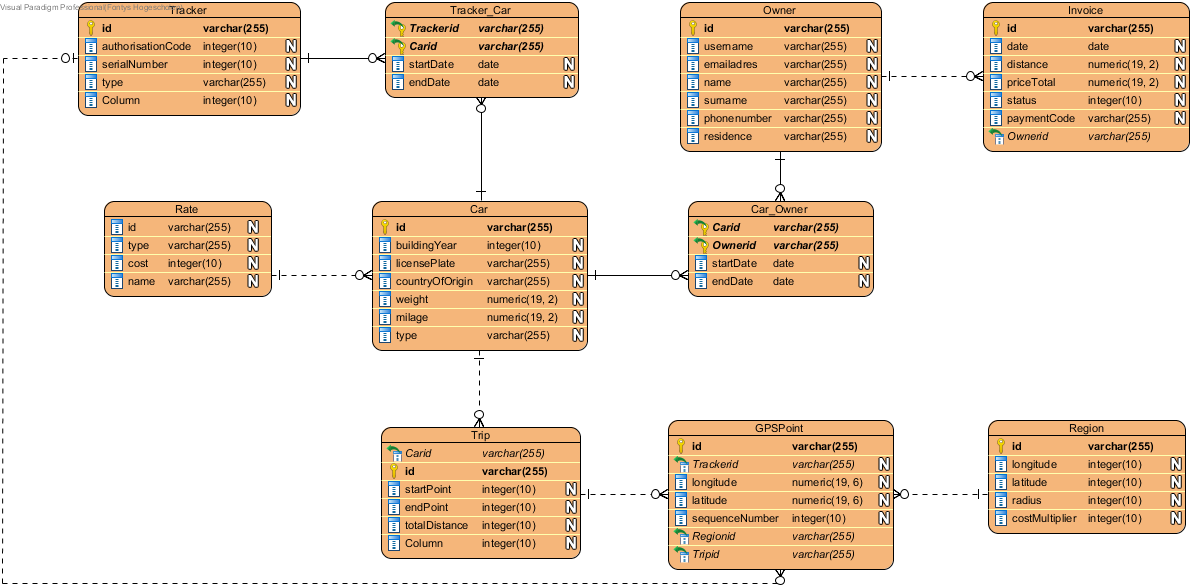
\includegraphics[draft]{erd-rekeningrijders}
		\label{fig:erd}
		\caption{Entiteiten Relatie Diagram}
	\end{figure}
		
	\section{Afbakening}
	
	\newpage
	\chapter{Persistentie}
		De persistentie vind plaats door middel van een Postgress database. Deze zal in de productie omgeving met meerdere replicaties werken om de prestatie en redundancy te verbeteren, maar in de productie draait het op een enkele database voor de simpliciteit.\par
		De authenticatie maakt gebruik van een OpenLDAP server, deze slaat alleen de authenticatie gegevens van de gebruiker op. De wachtwoorden zijn opgeslagen met het SHA algoritme om te zorgen dat wachtwoorden niet uit te lezen zijn.\par
	\newpage
	\chapter{Communicatie}
		De communicatie verloopt via een opgesteld HTTP Rest protocol waarmee alle onderdelen beschikbaar zijn. Op deze gegevens rust echter wel een beveiliging zodat alleen de gebruikers die er recht op hebben deze gegevens kunnen inzien. Deze authenticatie verloopt via HTTP Basic authenticatie.
		%TODO bescrijving api endpoints
	
	\newpage
	\chapter{Realisatie niet-functionele eisen}
	\section{Betrouwbaarheid}
	\section{Performance}
	\section{Beveiliging}
		De verbindingen zullen in de productie omgeving beveiligd worden door middel van SSL/TLS. Dit zorgt ervoor dat het praktisch onmogelijk is om als buitenstaander de communicatie af te luisteren.
	\section{Schaalbaarheid}
	
	\newpage
	\chapter{Componenten}
	\section{Componenten Diagram}
	\begin{figure}[ht]
		\centering
		\includegraphics[draft]{component-diagram}
		\label{pic:component-diagram}
		\caption{Componenten Diagram}
	\end{figure}
	\section{Koppeling tussen componenten}
	\section{Synchronisatie tussen componenten}
	\section{Services per component}
	\section{Allocatie van objecten}
	\section{Remote objecten}
	\section{Packagestructuur}
	
	\newpage
	\chapter{Deployment}
	\section{Deploymentdiagram}
	\begin{figure}[ht]
		\centering
		\includegraphics[draft]{deployment-diagram}
		\label{pic:deployment-diagram}
		\caption{Deployment Diagram}
	\end{figure}
	
	\newpage
	\chapter{Specificatie van interfaces}
\end{document}